%!TEX root = ../thesis.tex

% ------------------ Literature ------------------ %
Langran 1989
Peuquet 1994
Wachowitz 1999
Yuan 1999
Peuquet 2002

% http://link.springer.com/article/10.1007/s12145-009-0027-6/fulltext.html
% http://stackoverflow.com/questions/5863676/table-design-for-spatio-temporal-data

Multidimensional Geographic Information Science (Raper, 2001)
\cite{raper2000multidimensional}

whole book:
\cite{Langran1989timeingis}

chapters:
1 Fuzzs Sets ...
Spatio-Temporal Databases (Caluwe et al, 2010)
-> ontology of imperfection
\cite{deCaluwe:2010:SDF:1965517}


% ------------------------------------------------------------------------------
HGIS react on the spatial turn of history: the integration of geographic methods in historical research. It aims to discover the power of cartographic representation: ``The spatial turn in the humanities must [...] understand the role of space in human events''
\cite{bodenhamer2010spatial}.
At the same time, they are the product of the temporal run in GIS: the coexistence of space (where things are) and time (what has changed over time)
\cite[p. 45]{solana2014spatio}.

Since ``the world never stands still'', but ``the retention of information relating to past events [is] an important element of human representation of the world'', the dimension of time has to be integrated into a GIS
\cite{peuquet99}.

HGIS are rather recent tools and used mostly in \emph{Digital Humanities} as a digital tool to answer research questions in the traditional fields of humanities: ``situating history in its geographical context and using geographic information to illuminate the past''
\cite[p. 3]{knowles2008placing}.
Some interesting research questions that could be answered using HGIS could be:

\begin{compactitem}
  \item Did the European Union help to bring peace on the European continent?
  \hfill \emph{(political)}
  \item Is there a coherence between life expectancy and fertility rate?
  \hfill \emph{(social)}
  \item What is the effect of global warming on the melting of glaciers?
  \hfill \emph{(physical)}
  \item What was the effect of Bismarck's foreign policy on peace in Europe?
  \hfill \emph{(historical)}
\end{compactitem}

Or on a more abstract level: Where and When has something changed and why did it change?

\begin{enumerate}
  \item \textbf{Input}: Primary acquision of spatio-temporal data, i.e.\ historical events, historical and current countries and their territories.
  \item \textbf{Management}: Physical storage and logical management of the data in a spatio-temporal database, using a structure that fits the spatio-temporal data model.
  \item \textbf{Analysis}: Gaining spatio-temporal information by cleaning, transforming or combining the data in database.
  \item \textbf{Presentation}: Visualization of information on different displays, e.g.\ a map and a timeline, transforming information into spatio-temporal knowledge.
\end{enumerate}

% ------------------------------------------------------------------------------

A famous visualization combining time and space is ``Napoleons Moscow Campaign'' by Charles Minard from 1869 (see figure \ref{fig:minard_napoleon}). The ``best statistical graphic ever drawn''
\footnote{
  \emph{The Visual Display of Quantitative Information} (p. 40),
  Edward R. Tufte,
  2001
}
shows the size of the army in Napoleon’s 1812 Russian campaign, their movements and temperature on in one graph
\cite[pp. 188-191]{knowles2008placing}.

\begin{figure}[ht]
  \centering
  \includegraphics[width=0.8\textwidth]{graphics/basics/napoleon_march_moscow.png}
  \caption{Napoleons Moscow Campaign \protect\footnotemark}
  \label{fig:minard_napoleon}
\end{figure}

\footnotetext{
  \emph{Minard.png}
  Charles Minard, 1869,
  URL: \url{https://commons.wikimedia.org/wiki/File:Minard.png},
  accessed on: 03.11.2015,
}

==============================================================================


temporal domain
  linear time
    time line
    time series: graph (t,y coordinate system)
    2.5D map: temporal dimension on z axis or on surface
    space-time path
  cyclic time
    time series: polar diagram
    time wheel
  both
    mono-temporal: one layer -> one time point
    multi-temporal: one layer -> multiple time points
\cite[p. 144]{ott2001time}

paragraph timelines (end)


- - - - - - - - - - - - - - - - - - - - - - - - - - - - - - - - - - - - - - -
\paragraph{Geospatial Topology} % (fold)
\label{par:geospatial_topology}

\emph{Topology} is the study of position, how objects are spatially arranged and relatively positioned to each other. It does not include measures like distances or angles. Two objects are said to be topologically equivalent, if they can be deformed into each other, e.g.\ an ellipse can be stretched into a circle. A \emph{geospatial topological vector model} defines the relationship between geospatial objects, i.e.\ equals, disjoint, intersects, touches / neighbors, contains, covers, within, interior and boundary
\cite{clementiniTopology}.

The 2D vector model can be extended with a topology. The elements in this topological space are nodes (0D), edges (1D) and meshes (2D) and they correspond directly to the geometric primitives stated above. A topological vector model has strict connectivity (a ``clean'' geometry), if no two edges intersect without a node at their intersection point (planar), each interior edge has exactly two adjacent areas and each edge contains at least two nodes
\cite[pp.37-39]{bolstad2008gis}.

\begin{figure}[ht]
  \centering
  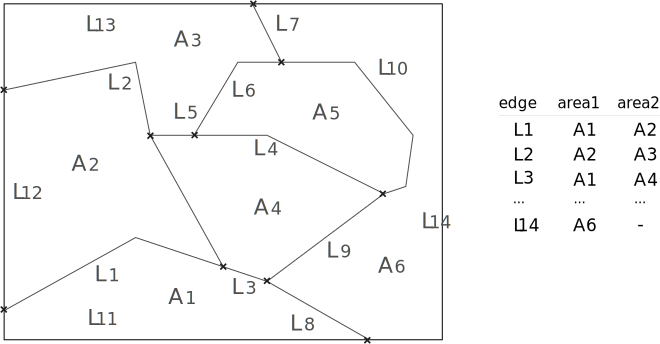
\includegraphics[width=0.55\textwidth]{graphics/basics/topological_vector_model}
  \caption{An example of a topological vector model and an adjacancy table}
  \label{fig:topological_vector_model}
\end{figure}

The topological vector model has a great asset: if an edge between two adjacent areas changes, the connectivity and adjacency does not change and therefore also the topology stays constant. The lookup for neighboring areas is very fast if the topology ensures strict connectivity: The neighbors of an area can be found in the adjacency table. Potentially problematic is the creation of a clean geometry: it can be cumbersome and require a lot of manual adjustment, for example ensuring strict connectivity by manually connecting nodes.

% paragraph geospatial_topology (end)

% subsection model_of_geographical_space (end)


\begin{figure}[H]
  \centering
  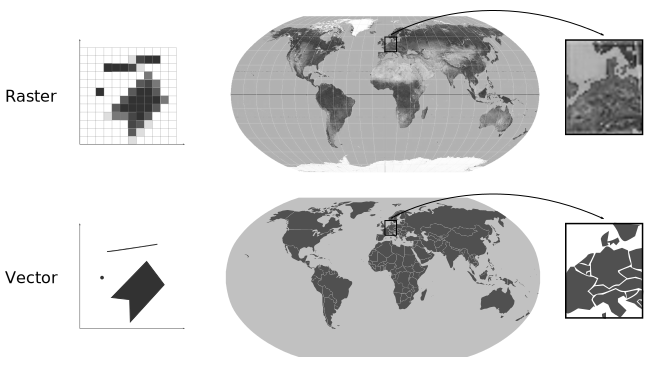
\includegraphics[width=0.75\textwidth]{graphics/basics/hgis/raster_vector}
  \caption{Comparison of the raster and the vector model}
  \label{fig:raster_vector}
\end{figure}

The \emph{raster model} contains a regular grid with a fixed \emph{cell dimension}. Each cell has a certain value, e.g.\ a color value.
The model is simple and allows straightforward rendering: only affine transformations have to be applied in order to project two raster map layers on top of each other. The main disadvantage of the raster model is its fixed resolution: it cannot be scaled up without losing quality
\cite[pp.42-48]{bolstad2008gis}.
Raster graphics are used for map tiles by most map engines, e.g.\ the satellite image by NASA in Google Maps.
\footnote{
  \emph{Google Maps},
  URL: \url{https://www.google.com/maps/@51.2090662,13.2328189,3563505m/data=!3m1!1e3},
  Imagery \textcopyright2015 Landsat, Data SIO, NOAA, U.S. Navy, NGA, GEBCO, IBCAO, U.S. Geological Survey, Map data \textcopyright2015 Google, ORION-ME,
  accessed on: 29.10.2015
}.


For time spans, there are six possibile temporal topological relations (table \ref{tab:temporal_relations}). Except for \texttt{equals}, each of them has an inverse, yielding a total of 13 different relations.

\begin{table}[H]
\begin{center}
\begin{tabular}{c c c}
    % \toprule
    relation & symbol & visualization \\
    \midrule
    $X$ before $Y$ &    \texttt{X < Y} & \raisebox{-0.25\height}
    {
\includegraphics{graphics/basics/temporal_relations/before}} \\
    $X$ meets $Y$ &     \texttt{X m Y} & \raisebox{-0.25\height}
    {\includegraphics{graphics/basics/temporal_relations/meets}} \\
    $X$ overlaps $Y$ &  \texttt{X o Y} & \raisebox{-0.25\height}
    {\includegraphics{graphics/basics/temporal_relations/overlaps}} \\
    $X$ equals $Y$ &    \texttt{X = Y} & \raisebox{-0.25\height}
    {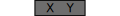
\includegraphics{graphics/basics/temporal_relations/equals}} \\
    $X$ starts $Y$ &    \texttt{X s Y} & \raisebox{-0.25\height}
    {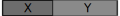
\includegraphics{graphics/basics/temporal_relations/starts}} \\
    $X$ during $Y$ &    \texttt{X d Y} & \raisebox{-0.25\height}
    {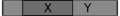
\includegraphics{graphics/basics/temporal_relations/during}} \\
    $X$ ends $Y$ &      \texttt{X e Y} & \raisebox{-0.25\height}
    {
\includegraphics{graphics/basics/temporal_relations/ends}} \\
    % \bottomrule
\end{tabular}
\caption{Temporal relations of time spans, based on \cite{allen84}}
\label{tab:temporal_relations}
\end{center}
\end{table}

% paragraph temporal_relations (end)

% ==============================================================================
\section{Database Management Systems} % (fold)
\label{sec:database_management_systems}

Information systems use databases for managing the data. A \emph{Database Management System} (DBMS) is a software system for the administration of data, mainly storage and retrieval. There are mainly two types of DBMS: the oldest and most common ones are \emph{Relational DBMS}. \emph{Object-Oriented DBMS} werde developed to adapt concepts of object-oriented programming into the database world. The combination of both approaches are \emph{Object-Relational DBMS}.

% ------------------------------------------------------------------------------
\subsection{Relational Database Management Systems} % (fold)
\label{sub:relational_database_management_systems}

RDBMS are built upon the concept of \emph{entitities}, e.g.\ an \texttt{HistoricalCountry}, with \emph{attributes}, e.g.\ \texttt{name} and attribute values of a simple data type, e.g.\ the character string \texttt{"Germany"}. Entities are represented in a table with one row for each \emph{tuple} and one column for each attribute. An entity has one attribute that unambiguously identifies each tuple, the \emph{primary key}, mostly a contiguous number.

Entities can be related to each other in three different kinds of \emph{relations}:
\begin{compactenum}
  \item[\texttt{1:1}] Direct attributional relation, e.g.\ one country has one head of state and vice versa.
  \item[\texttt{1:n}] One-to-many relation, e.g.\ one country can have many cities, but each city can belong to only one country.
  \item[\texttt{m:n}] Many-to-many relation, e.g.\ one country can have many rivers, but each river can also flow through multiple countries.
\end{compactenum}

Entities and their relations are visualized in an \emph{Entity-Relationship Model} (ER model). Data can be retrieved from and entered into a relational database using the \emph{Structural Query Language} (SQL). The query to get the names of cities in \texttt{Germany} in alphabetical order is:

\vspace{-1em}
\begin{verbatimtab}
  SELECT     city.id, city.name
  FROM       (city JOIN country ON city.country = country.id)
  WHERE      country.name = "Thüringen"
  ORDER BY   city.name
\end{verbatimtab}
\vspace{-1em}

The first RDBM developed was \emph{Oracle}, released in 1979 \cite{oracleDB}. Since then, the concept has been established as the state-of-the-art for databases. An example for a popular RDBMS used for Web-bases systems is \emph{MySQL}, the ``world's most popular open source database''
\footnote{
  \emph{MySQL :: About MySQL},
  URL: \url{https://www.mysql.com/about/},
  accessed on: 31.10.2015
}.


% subsection relational_database_management_systems (end)

% ------------------------------------------------------------------------------
\subsection{Object-Oriented Database Management Systems} % (fold)
\label{sub:object_oriented_database_management_systems}

One problem with RDBMS is that attributes can only be assigned simple data types. Developers using object-oriented programming need to map the objects used in the application to tuples in the relational database -- and vice versa data from the database needs to be transformed to objects in the application. This process can be cumbersome. OODBMS have been developed to address this problem and adopt the concepts of object-oriented programming for database management purposes \cite{oodbms}.

\begin{itemize}
  \item \emph{Classes} are the structured representation of things in the real world of the same kind, with the same properties, e.g.\ a country, having a name and a territory. Classes in OODBMS relate to Entities in RDBMS.
  \item An \emph{object} is an instance of a class, one specific thing with defined properties, e.g.\ the country of Germany with its territory. This correlates to a tuple in RDBMS.
  \begin{itemize}
    \item The \emph{attributes} of an object cannot just be of a simple data type, but also instances of other classes, e.g.\ \texttt{country.territory} can be a \texttt{polypolygon} object. These complex data types are a major improvement compared to RDBMS.
    \item Objects also have \emph{methods} that can be called to do something with the object, e.g.\ \texttt{territory.getArea()} calculates the area size of a country.
  \end{itemize}
  \item The internal state of an object cannot be accessed from the outside. Methods are the only way to interact with an object. This is called \emph{encapsulation} and maintains control over what can be done to and with an object and prevents corruption.
  \item According to the concept of \emph{inheritance}, classes can be hierarchically structured, whereas the attributes and the methods of a \emph{base class} are inherited to its \emph{derived class}. As an example, an \texttt{Area} has a \texttt{name}, a \texttt{territory} and the method \texttt{getArea()} associated to it. A \texttt{Country} can be derived from the \texttt{Area}, inheriting both attributes and the method. Additionally, it can get an attribute \texttt{head\_of\_state}, which is specific to \texttt{Country}, but not to \texttt{Area}. The class \texttt{Ocean} can just as well be derived from \texttt{Area}.
  \item An associated concept is \emph{polymorphism}: The same function can be called on different objects and the return value will be of the same type. However, internally it might be calculated differently. As an example, consider the classes \texttt{Polygon} and \texttt{Polypolygon}, both inherited the method \texttt{getArea()} from their base class \texttt{Geometry}. Whereas a polygon calculates its area directly based on its geometry, a polypolygon internally calles the function \texttt{getArea()} on all its associated polygons and sums up their areas.
\end{itemize}

OODBMS support all those concept and allow to store the objects used in the application directly in the database. Additionally, objects from the database can be accessed directly, there is no need for an additional query language \cite{oodbms}.

% subsection object_oriented_database_management_systems (end)

% ------------------------------------------------------------------------------
\subsection{Object-Relational Database Management Systems} % (fold)
\label{sub:object_relational_database_management_systems}

ORDBMS combine the advantages of both worlds. Internally, it uses the established and efficient relational database for the data storage. The database model and the interaction with the data happens in an object-oriented way while supporting all of the concepts mentioned in the previous subsection \ref{sub:object_oriented_database_management_systems}. The most popular ORDBMS example for Web-based systems is \emph{PostgreSQL}, ``the world's most advanced open source database''
\footnote{
  \emph{PostgreSQL:},
  The world's most advanced open source database,
  URL: \url{http://www.postgresql.org/},
  accessed on: 31.10.2015
}.

% subsection object_relational_database_management_systems (end)

% ------------------------------------------------------------------------------
\subsection{Spatio-Temporal Databases} % (fold)
\label{par:spatial_databases}

Databases for HGIS have to deal with spatial, temporal and attribute data. According to the Triadic Frame, these aspects should be modeled separately from each other, as they can change independently.

% - - - - - - - - - - - - - - - - - - - - - - - - - - - - - - - - - - - - - - -
\paragraph{Spatial data} % (fold)
\label{par:spatial_data}

can easily become very large, because of the mass of very precise coordinate data. \emph{Spatial databases} are specialized to work with spatial data: they process the data effieciently and to provide general data types, such as \texttt{Point} or \texttt{Polygon} and methods, e.g.\ to calculate the area or the distance between two points. \emph{PostGIS}
\footnote{
  \emph{PostGIS},
  URL: \url{http://postgis.net/},
  accessed on: 31.10.2015
}
is an extension for PostgreSQL that is especially utilized for handling spatial data.

% paragraph spatial_data (end)


% - - - - - - - - - - - - - - - - - - - - - - - - - - - - - - - - - - - - - - -
\paragraph{Temporal data} % (fold)
\label{par:temporal_data}

usually relates to events and processes. It is defined either by a time point or a time interval which is again defined by two time points. This is called a \emph{bitemporal} element. A time point can be modeled in the database as an attribute of the complex \texttt{Date} type. For relational databases that only support simple data types, the date can be stored as a string or be expressed with a \texttt{long} integer (64 bit) $\forall n \in \mathbb{N}: n \in [-2^{63}~..~2^{63}-1]$) determining the number of milliseconds since \nth{1} January 1970 (UNIX time) \cite{timeInRDBMS}. SQL was extended by features to handle time in a database, e.g.\ \emph{SQL/MM} \cite[chapter 6]{peuquet99}.

% paragraph temporal_data (end)

% - - - - - - - - - - - - - - - - - - - - - - - - - - - - - - - - - - - - - - -
\paragraph{Object-Oriented Spatio-Temporal Database Models} % (fold)
\label{par:object_oriented_spatio_temporal_database_models}

The question is: How to implement the spatio-temporal data modles introduced in section \ref{sec:spatio_temporal_data_models} in a relational, object-oriented or object-relational database management system introduced in this section? While the implementation depends on the data model, there are common concepts and isses that have to be addressed.

When storing time related data, it is important to distinguish between the time that was true in reality (\emph{valid time} or \emph{world time}) and the time it was stored in the database (\emph{transaction time} or \emph{database time}). A property of spatio-temporal database models is whether valid and transaction time are supported.

Object-oriented concepts are more appropriate than the concept of relational databases, because of the complex nature of spatio-temporal data \cite[section 3.9]{pelekis04stdms}. One of the first concepts was the concept of a \emph{spatio-temporal object} combining geometrical and bitemporal properties in one object \cite{worboys90stdm}.

A similar approach by \cite{raza12} is the \emph{Spatio-Temporal Data Type} (STT). Time is not considered an attribute of space, but a separate class. They are aggregated in the \texttt{SpatioTemporal} class, using both spatial and bitemporal attributes. The model also provides spatio-temporal operators, e.g.\ \texttt{STT\_intersects} returns \texttt{true} if two \texttt{SpatioTemporal} objects intersect in time and space, i.e.\ their geometries intersect and the time intervals in which they are active overlap. These operators are very helpful when analyzing spatio-temporal data or checking for data integrity.

% paragraph object_oriented_spatio_temporal_database_models (end)

% - - - - - - - - - - - - - - - - - - - - - - - - - - - - - - - - - - - - - - -
\paragraph{Version management} % (fold)
\label{par:version_management}


One approach to handle this issue is \emph{version management}, introduced by
\cite WH94
There are \emph{object version} and \emph{object configuration}. The concept is based on four premises:
\begin{compactenum}
  \item Each object must have an initial version.
  \item The versions of an object are hierachically structured.
  \item One object version relates to exactly one object instance and vice versa.
  \item There is always one current version of an object.
\end{compactenum}

Throughout time, a set of interrelating object versions is created. They are handled by four update procedures that create new object versions:
\begin{compactenum}
  \item Create of a new object.
  \item Clone an existing object.
  \item Update spatial attributes of an existing object (geometric change).
  \item Update aspatial attributes of an existing object (thematic change).
\end{compactenum}

paragraph version_management (end)


\cite[p. 69]{ott2001time}.

section database_management_systems (end)
